\documentclass[12pt,a4paper]{article}
\usepackage{cmap}
\usepackage{mathtext}
\usepackage{amssymb}
\usepackage{amsmath}
\usepackage[russian]{babel}
\usepackage{indentfirst}
\usepackage[pdftex]{graphicx}
\usepackage{multirow}
\usepackage{mathrsfs}
\usepackage{biblatex}
\usepackage{siunitx}
\usepackage[left=2cm,right=2cm,top=2cm,bottom=2cm]{geometry}
\usepackage{fancyhdr}
\usepackage{floatrow,calc}

\bibliography{bib}
\pagestyle{plain}
\newcommand{\rref}[1]{(\ref{#1})}
\newenvironment{comment}{}{}
\newcommand{\picref}[1]{рис. \ref{#1}}
\newcommand{\mbf}{\mathbf}
\newcommand{\Equip}[3]{
	
	{\bf #1:} $\Delta = \pm #2$ \si{#3}}
\newcommand{\equip}[1]{
	
	{\bf #1}}
\begin{document}
\title{\begin{center}Лабораторная работа № 4.1.1\end{center}
Геометрическая оптика}
\author{Струков О. И. \\ Б04-404}
\date{}

\thispagestyle{empty}
\pagenumbering{gobble}
\maketitle
\newpage
\pagenumbering{arabic}
\section*{Введение}
В данной работе проводится изучение методов определения фокусных расстояний линз и сложных оптических систем, а также определение характеристик оптической системы, составленной из тонких линз; производится изучение недостатков реальных линз — сферической и хроматической аберраций.
\section*{В работе используются:}

Линейка,
Оптическая скамья с набором рейтеров,
Положительные и отрицательные линзы,
Экран,
Осветитель с ирисовой диафрагмой,
Зрительная труба,
Светофильтры,
Кольцевые диафрагмы.

\section*{Теоретическая часть}


Используя закон преломления, получим для элементарной оптической ячейки, изображённой на \picref{2}, в параксиальном приближении:
\begin{equation}\label{опт-ячейка}
	-\frac{n}{x}+\frac{n'}{x'} = \frac{n'-n}{R},
\end{equation}
\begin{equation}
	x \alpha = x' \alpha'.
\end{equation}
Для прямой $ P P' $, рассмотренной как оптическая ось, 
\begin{equation}\label{PP}
	\frac{y'}{y} = \frac{x' - R}{x - R}.
\end{equation}

Проведя замену переменных, получим систему уравнений
\begin{equation}\label{grid}
	\frac{x' - F'}{H' - F'}= \frac{H-F}{x- F} = \frac{y'}{y} = \frac{n \alpha}{n' \alpha'},
\end{equation}
\begin{equation}\label{grid1}
	(x-H)\alpha= (x' - H')\alpha'.
\end{equation}
Из этих уравнений получим
\begin{equation}\label{Ф}
	\frac{n}{f} = -\frac{n'}{f'} \equiv \Phi,
\end{equation}
где
\begin{equation}\label{focus-len}
	f\equiv H - F, \;\;\; f'\equiv H' - F'.
\end{equation}
$ f $ и $ f' $ -- главные фокусные расстояния системы.

\begin{figure}[H]
	\centering
	
\includegraphics[width=0.8\linewidth]{Screenshot_1}
	\caption{Элементарная оптическая ячейка}
	\label{2}
\end{figure}



\subsection*{Определение фокусного расстояния тонкой собирающей линзы и сложных оптических систем по методу Аббе}

Схема, применяемая для определения фокусного расстояния $ F $ оптической системы по методу Аббе, изображена на \picref{1}.
\begin{figure}[tbp]
	\centering
	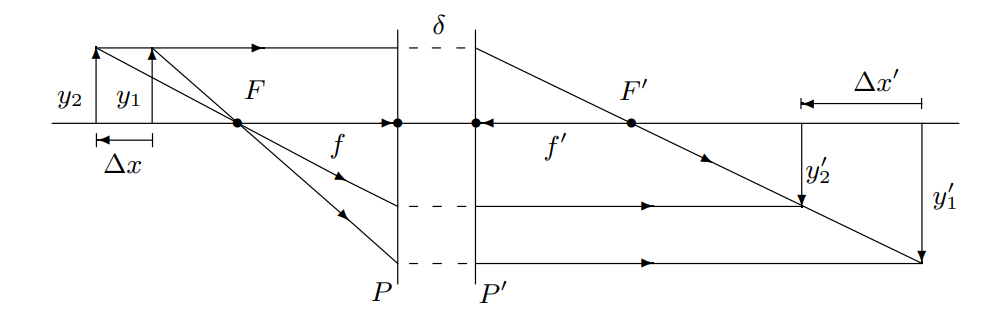
\includegraphics[width=0.8\linewidth]{Screenshot_3}
	\caption{Иллюстрация метода Аббе}
	\label{1}
\end{figure}

Из формул \eqref{Ф}, \eqref{grid}, \eqref{focus-len} получим:
\begin{equation}\label{abbe}
	f = \frac{\Delta x}{\Delta (y/y')} = -\frac{\Delta x'}{\Delta (y'/y)}.
\end{equation}

\subsection*{Определение фокусного расстояния собирающих линз и сложных оптических систем по методу Бесселя}

\begin{figure}[tbp]
	\centering
	
\includegraphics[width=0.8\linewidth]{Screenshot_2}
	\caption{Иллюстрация метода Бесселя}
	\label{3}
\end{figure}
Схема метода Бесселя для случая, когда $n = n'$ и $f' = -f$, представлена на \picref{3}. Тогда фокусное расстояние вычисляется по формуле:
\begin{equation}\label{Bessel}
	f = \frac{(L - \delta)^2 - l^2}{4(L-\delta)}.
\end{equation}

В данной работе предпочтение отдаётся методу Аббе.

\subsection*{Определение фокусного расстояния тонкой собирающей линзы}

\paragraph{Способ 1.} Воспользуемся формулой тонкой линзы:
\begin{equation}\label{thin-lens}
	-\frac{1}{a}+\frac{1}{a'} = \frac{1}{f}.
\end{equation}
\paragraph{Способ 2.}
Фокусное расстояние тонкой собирающей линзы можно определить с помощью зрительной трубы, настроенной на бесконечность, то есть на параллельный пучок лучей. Разместив между предметом и зрительной трубой положительную линзу и перемещая её вдоль оси системы, можно найти резкое изображение предмета в окуляре зрительной трубы. При этом расстояние от середины линзы до предмета равно фокусному расстоянию тонкой линзы.

\subsection*{Определение фокусного расстояния тонкой рассеивающей линзы}

\paragraph{Способ 1.} Сначала с помощью собирающей линзы получают на экране действительное изображение предмета $ S $ (точка $ S_1 $ на \picref{4}). Затем на пути лучей, выходящих из собирающей линзы, располагают исследуемую рассеивающую линзу и, отодвигая экран, получают чёткое изображение предмета на экране, образованное двумя линзами. Точка $ S_1 $ пересечения сходящихся лучей играет по отношению к рассеивающей линзе роль мнимого источника. Изображение источника переместится теперь в точку $ S_2 $. 

\begin{figure}[tbp]
	\centering
	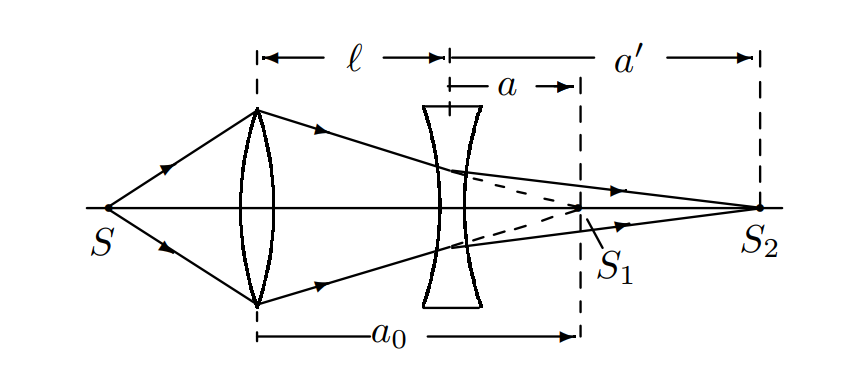
\includegraphics[width=0.8\linewidth]{Screenshot_5}
	\caption{Определение фокусного расстояния тонкой рассеивающей линзы}
	\label{4}
\end{figure}


Определив расстояния $ a = a_0 - l > 0$ и $ a'>0 $, рассчитывают фокусное расстояние рассеивающей линзы по формуле \eqref{thin-lens}.

\paragraph{Способ 2}

Если расстояние $ a $ на \picref{4} совпадает с модулем фокусного расстояния рассеивающей линзы, то изображение $S_2$ перемещается в бесконечность, то есть лучи выходят из линзы параллельным пучком. Параллельность пучка можно установить с помощью зрительной трубы, настроенной на бесконечность. Зная расстояние от первой линзы до точки $S_1$ и расстояние между линзами, нетрудно определить фокусное расстояние тонкой рассеивающей линзы. Для толстой отрицательной линзы этот метод позволяет определить только положение главного фокуса.


\subsection*{Определение положения главных и фокальных плоскостей сложной оптической системы}

Для нахождения главных плоскостей системы недостаточно знать фокусное расстояние, нужно определить ещё положения главных фокусов. Это можно сделать при помощи зрительной трубы, настроенной на бесконечность. Отложив от главных фокусов отрезки, равные фокусному расстоянию, можно найти положения главных плоскостей системы. При этом необходимо учитывать возможность различного взаимного расположения кардинальных точек (плоскостей) сложной системы.






\section*{Ход работы}

\subsection*{Определение фокусных расстояний линз с помощью подзорной трубы}

Подзорная труба была сфокусирована на ``бесконечность'', а собирающие линзы располагались между ней и источником. В тот момент, когда в подзорную трубу было видно чёткое изображение, из линзы выходил параллельный пучок лучей, а расстояние между ней и источником равнялось фокусному.

Фокусное расстояние рассеивающей линзы определялось с помощью создания системы с одной из собирающих линз.

При развороте линз фокусное расстояние совпадало с измеренным ранее, из чего следует, что их можно считать тонкими линзами.


\begin{table}[H]
\begin{tabular}{|c|c|}
\hline
Номер линзы & f, см \\ \hline
1           & 8     \\ \hline
2           & 13    \\ \hline
3           & 17,7  \\ \hline
4           & 25    \\ \hline
5           & -22   \\ \hline
6           & 5     \\ \hline
\end{tabular}
\end{table}


\subsection*{Измерение фокусных расстояний линз по формуле тонкой линзы и методом Бесселя}

Для изучения была выбрана линза номер 2 с фокусным расстоянием 13 см. Экран был помещён расстоянии L = 70 см от источника.
Исследуемая линза была помещена между экраном и источником, и были определены два её положения относительно источника $a_1$ и $a_2$, при которых на экране возникают чёткие изображения.

Фокусные расстояния $f_1$ и $f_2$ были вычислены с помощью формулы тонкой линзы
\[ \dfrac{1}{f} = \dfrac{1}{a} + \dfrac{1}{L - a} \]
Фокусное расстояние $f_3$ было вычислено по приближённой формуле Бесселя
\[ f \approx \dfrac{L^2 - l^2}{4L} \]
Как видно, результаты, представленные в таблицах ниже, достаточно близки друг к другу и совпадают в пределах погрешностей:


\begin{table}[H]
\begin{tabular}{|c|c|c|c|c|c|}
\hline
$а_1$, см      & $а_2$, см      & $l$, см    & $f_1$, см    & $f_2$, см   & $f_3$, см    \\ \hline
$16,2\pm0,1$ & $53,9\pm0,1$ & $37,7\pm0,2$ & $12,45\pm0,13$ & $12,40\pm0,10$ & $12,42\pm0,15$ \\ \hline
\end{tabular}
\end{table}

После разворота линзы:
\begin{table}[H]
\begin{tabular}{|c|c|c|c|c|c|}
\hline
$а_1$, см      & $а_2$, см      & $l$, см    & $f_1$, см    & $f_2$, см   & $f_3$, см    \\ \hline
$16,5\pm0,1$ & $53,9\pm0,1$ & $37,5\pm0,2$ & $12,61\pm0,13$ & $12,40\pm0,10$ & $12,48\pm0,15$ \\ \hline
\end{tabular}
\end{table}


\subsection*{Сборка и изучение подзорной трубы Кеплера}

Из набора была взята линза 4 в качестве коллиматора, линзы 1 и 3 в качестве объектива и окуляра.
Картина, наблюдаемая через коллиматор с помощью вспомогательной подзорной трубы была сфотографирована на телефон:

\begin{figure}[H]
	\centering
	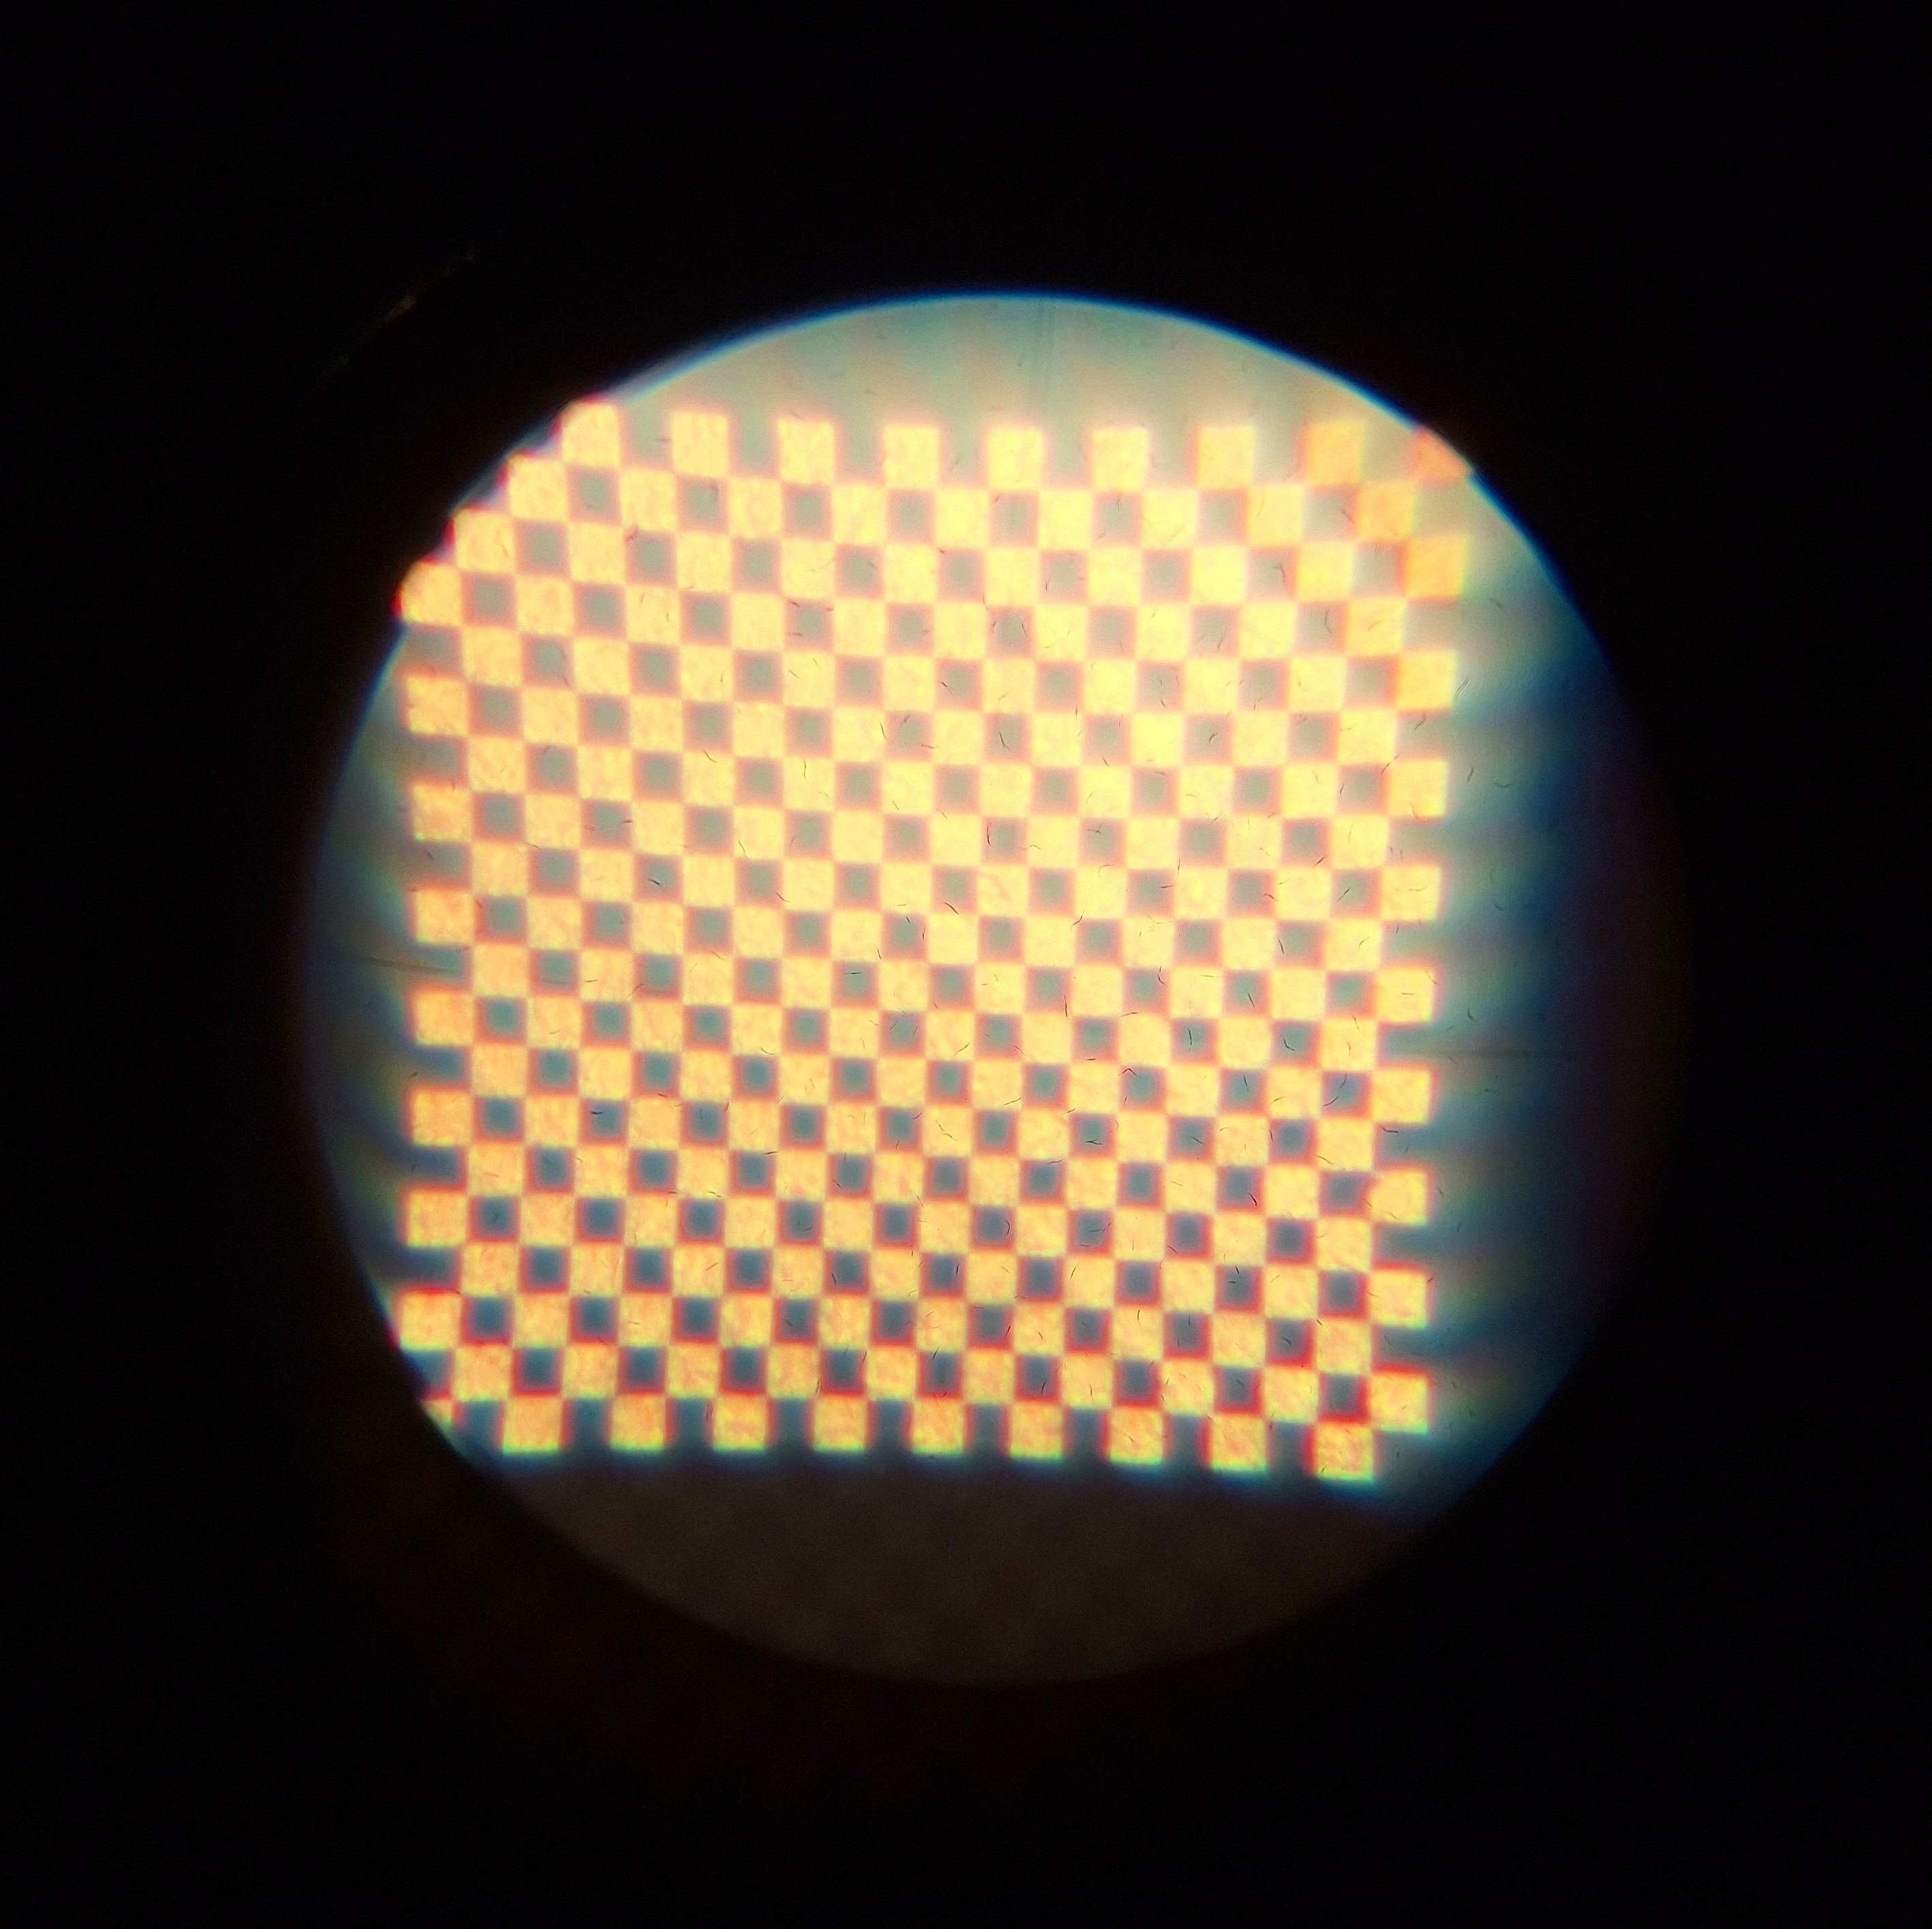
\includegraphics[width=0.6\linewidth]{Фото/20260305_104333.jpg}
	% \caption{Элементарная оптическая ячейка}
\end{figure}

После этого была собрана модель телескопа Кеплера по схеме на рисунке ниже

\begin{figure}[H]
	\centering
	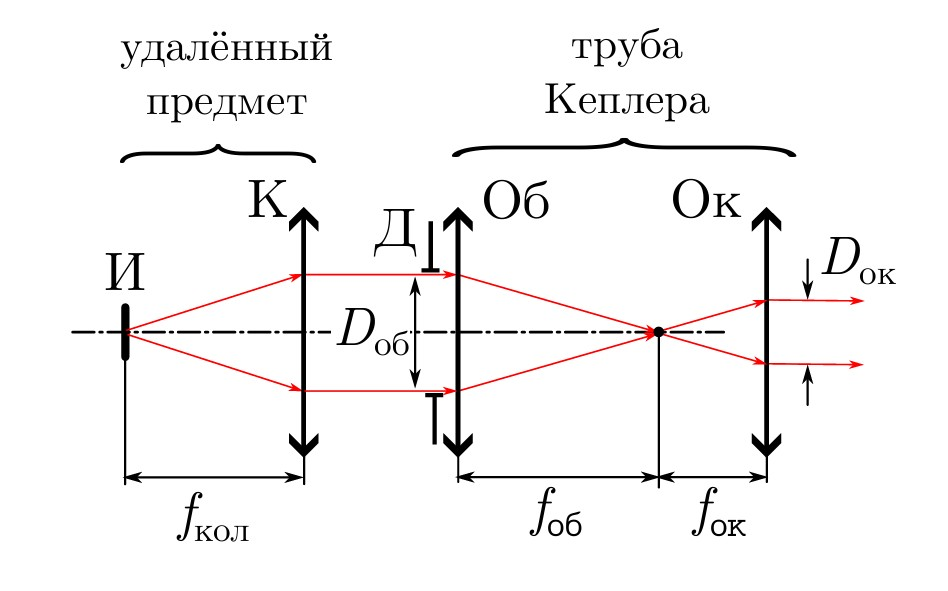
\includegraphics[width=0.6\linewidth]{Кеплер.jpg}
	% \caption{Элементарная оптическая ячейка}
\end{figure}

Полученное изображение было также сфотографировано, и с его помощью определено экспериментальное угловое увеличение $\gamma_{\text{эксп}} \approx 0,33$.
Теоретическое увеличение при этом составило $\gamma_{\text{}} = |f_{\text{об}} / f_{\text{ок}}| \approx 0,45$. Причинами расхождений могут быть неточно определённые фокусные расстояния линз и погрешности при их выставлении. 

\begin{figure}[H]
	\centering
	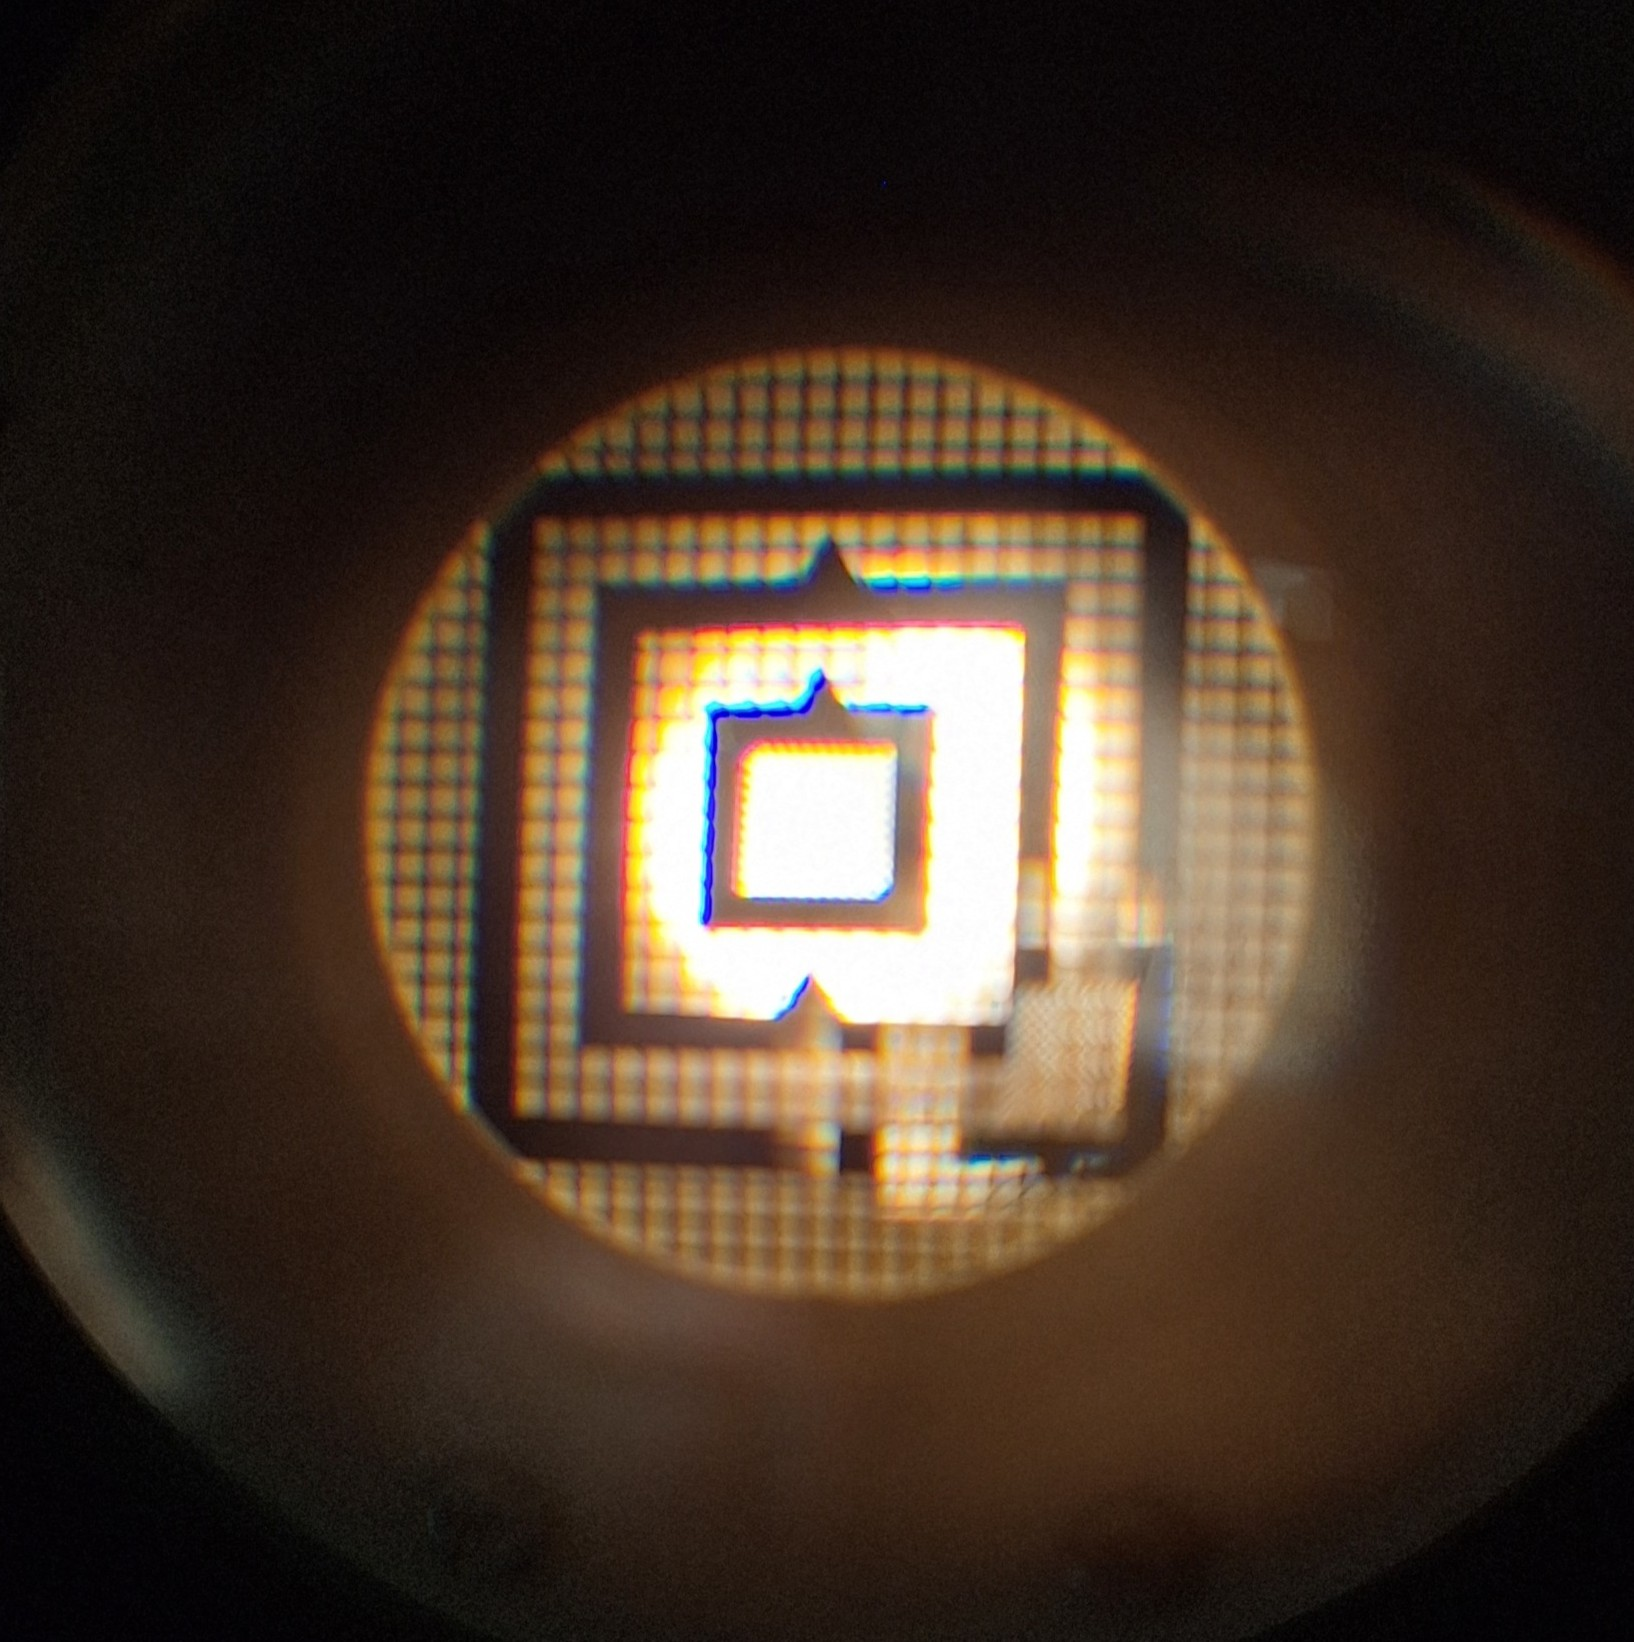
\includegraphics[width=0.6\linewidth]{Фото/20260305_105042.jpg}
	% \caption{Элементарная оптическая ячейка}
\end{figure}


\newpage
\subsection*{Сборка и изучение модели микроскопа}

Для сборки микроскопа были выбраны линзы номер 3 и 4. При заданном увеличении $\gamma \approx \dfrac{3}{5}$ из формулы $\gamma = \dfrac{\Delta L_{\text{зр}}}{f_{\text{об}} f_{\text{ок}}}$ была вычислена необходимая длина оптического интервала $\Delta = 10,62$ см.
По схеме ниже был собран микроскоп, и визуально полученное им увеличение было около 2, то есть близко к заданному значению 3/5.

\begin{figure}[H]
	\centering
	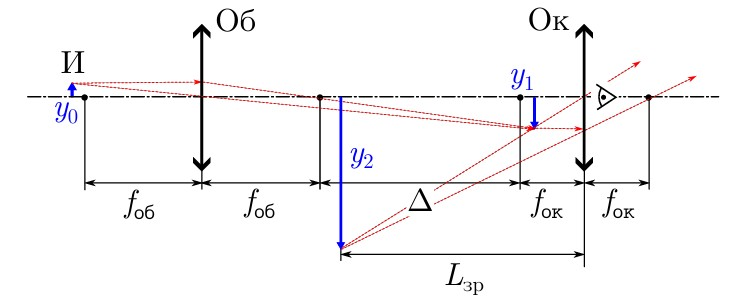
\includegraphics[width=0.6\linewidth]{Микроскоп.jpg}
	\caption{Наблюдение на расстоянии наилучшего зрения}
\end{figure}

Далее был собран проекционный микроскоп и получено сфокусированное изображение на экране. Его линейное увеличение составило $\Gamma = (1,22 \pm 0,09)$, что близко к рассчитанному теоретически $\Gamma_{\text{теор}}=1,38$.

\begin{figure}[H]
	\centering
	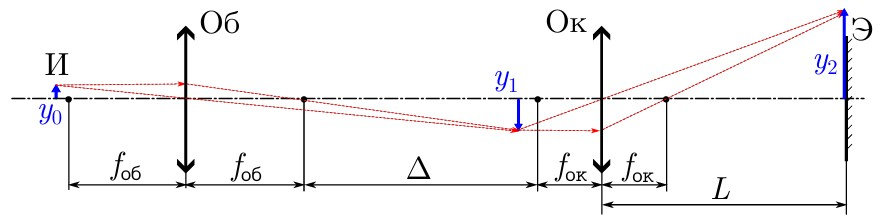
\includegraphics[width=0.6\linewidth]{Проекционный.jpg}
	\caption{Проекционный микроскоп}
\end{figure}

\subsection*{Изучение составной оптической системы}
Для эксперимента были взяты собирающая линза 1 и рассеивающая 5, которые были размещены подставками вплотную друг к другу. Фокусное расстояние системы составило $f = 11,8$ см.
Экспериментально было определено, что при расположении собирающей линзы ближе к источнику расстояние до фокуса составляет $f_b = 14,5$ см, а при расположении ближе рассеивающей -- $f_a = 7,7$ см.

Было проведено измерение фокусного расстояния $f$ и оптического интервала $\delta$ системы по методу Бесселя: система была расположена между источником и экраном,
расположенными на расстоянии $L>L_{min} = 4f$. При перемещении системы как целого между источником и экраном
измерялось её смещение $l$ между двумя чёткими изображениями (увеличенным и уменьшенным).
Измерения были проведены для 6 различных $L$ в диапазоне $L_{min} < L < 2 L_{min}$.

Чтобы найти фокусное расстояние из формулы Бесселя $l^2 = (L-\delta)(L-\delta-4f)$ на основе полученных измерений была построена зависимость $A(L) = L^2 -l^2  = 2L(\delta + 2f)-\delta^2 + 4\delta f$.
Отсюда $\delta = (3,84\pm0,61)$ см, $f=(8,76\pm0,48)$ см, что не совпадает с рассчитанным теоретически из-за неточного определения фокусных расстояний линз.

\begin{figure}[H]
	\centering
	
\includegraphics[width=1\linewidth]{График.pdf}
	\caption{График зависимости $A(L)$}
\end{figure}

\section*{Выводы}
В ходе работы были экспериментально определены фокусные расстояния собирающих и рассеивающих линз различными методами, полученные значения в большинстве случаев согласуются друг с другом в пределах погрешностей.
На основе изученных линз были собраны модели телескопа Кеплера и микроскопа (визуального и проекционного); их увеличения, определённые экспериментально, близки к теоретическим расчётам.
Для составной системы, состоящей из двух линз, методом Бесселя определены фокусное расстояние и оптический интервал, а также найдены положения главных плоскостей.%; наблюдаемое расхождение с теоретической оценкой объясняется неточностью исходных фокусных расстояний линз и погрешностью измерений.
% Таким образом, основные закономерности геометрической оптики и методы расчёта сложных систем успешно подтверждены экспериментально.



\end{document}